\chapter{Schlussfolgerung und Ausblick}
\label{Conclusion}
%Was wurde in dieser Arbeit gemacht? Was sind die wesentlichen Ergebnisse? Wo ist weiterer Forschungsbedarf? Welche interessanten Forschungsbereiche ergeben sich aus der eigenen Arbeit?

In dieser Arbeit wurde eine Parameterstudie zur Untersuchung von Stößen auf isotropen Platten durchgeführt. Zuerst wurde die benötigte Theorie in Kapitel~\ref{chap:Principles} hergeleitet. Anschließend wurden im Rahmen der Studie die Parameter in Tabelle~\ref{tab:VariierteParams} ausgehend vom Ausgangsfall in Tabelle~\ref{tab:Ausgang} variiert. In Kapitel~\ref{chap:Implementation} wurden die Veränderungen im Skript dargestellt und die Funktionsweise des Programmes erklärt. 

\begin{table}[H]
	\begin{center}
		\caption{Parameterstudie}
		\label{tab:VariierteParams}
		\begin{tabular}{l|c}
			\textbf{Variable} & \textbf{Wert}\\
			\hline
			$h$ & Höhe der Platte [cm]\\
			$v_{0}$ & Geschwindigkeit der Impaktors [cm/s]\\
			$r_{g}$ & Radius des Impaktors [cm]\\
			$\frac{\xi}{a}$ & Auftreffstelle in x-Richtung [entdimensioniert]\\
			$\frac{\eta}{b}$ & Auftreffstelle in y-Richtung [entdimensioniert]\\
			$Sv$ & $\frac{a}{b} \equiv \; \mbox{Seitenverhältnis der Platte}$ \\		
		\end{tabular}
	\end{center}
\end{table}

Wie in Kaptitel~\ref{chap:Durchfuehrung} ausgeführt, lassen sich einige Schlussfolgerungen aus den gewonnenen Ergebnissen ziehen. \\

\section{Anzahl der Aufschläge}
\label{sec:Aufschlag}

Interessant ist, dass die Anzahl der Aufschläge unter Einfluss der Auftreffgeschwindigkeit $v_{0}$ und des Radius' der Kugel $r_{g}$ nur von dem Massenverhältnis $Mr$ abhängt. Betrachtet man die Aufschläge unter Variation der Höhe, des Aufschlagortes oder des Seitenverhältnisses, haben die genannten Parameter einen messbaren Einfluss auf die Anzahl der Schläge. \\
Da die größte Kraft nicht immer beim Erstschlag auftritt, liegt es nahe, dass die Anzahl der Aufschläge und die mit ihnen verbundene Kraft für die Schadensbeurteilung wichtig sind.\\
Ebenfalls ist die Anzahl der Schläge direkt mit dem Abstand zum Rand der Platte beziehungsweise mit dem Abstand zum Mittelpunkt der Platte verknüpft. Mit steigender Steifigkeit zum Rand hin, sinkt die maximale Anzahl an Schlägen. Jedoch sind weder die maximale Kraft noch die maximale Durchbiegung in der Mitte der Platte vorzufinden. Da die kürzere der beiden Seiten einen größeren Einfluss auf die Plattensteifigkeit besitzt, sorgt ein erhöhtes Seitenverhältnis unter konstanter Fläche zu einer verkürzten Seitenlänge und somit sinken die Anzahl der Aufschläge mit dem Seitenverhältnis.
%@FINN: Vielleciht hier noch was dazu über die Anzahl der Aufschläge bei xi und eta

\section{Auslenkung der Platte}
\label{sec:Auslenkung}

Bei der Auslenkung spielt die Höhe der Platte eine zentrale Rolle. Vergrößert man $h$ während $Mr$ konstant gehalten wird, fällt die Auslenkung $w$ schnell ab. Allerdings ist $w$ bei geringem $h$ sehr groß, was durch induzierte Spannungen in der Platte Schäden hervorrufen kann.\\
Betrachtet man die Geschwindigkeit des Impaktors, wird schnell ersichtlich, dass hier $v_{0}$ der dominierende Parameter ist. Zwar steigt die Auslenkung mit größer werdendem $Mr$ an, jedoch ist diese Änderung wesentlich kleiner als der Anstieg bei konstantem $Mr$ und größer werdender Geschwindigkeit.\\
Der Radius der Kugel hat nur einen verschwindend geringen Einfluss auf die Auslenkung der Platte. Wie in Kapitel~\ref{chap:Durchfuehrung}, Abbildung~\ref{fig:RadiusAuslenkung} zu sehen ist, steigert sich die Auslenkung von $r_{g,min}$ zu $r_{g,max}$ nur in der zweiten Nachkommastelle. \\
Abbildung~\ref{fig:Faktoren} erhält man, indem man die maximalen und minimalen Auslenkungs- und Kraftwerte die bei $Parameter_{min}$ und $Parameter_{max}$ auftreten durcheinander teilt. Indem man dies jeweils für $Mr_{min}$ und $Mr_{max}$ macht, erhält man einen Überblick über den Einfluss des betrachteten Parameters.\\
Zu beachten ist hier, dass bei Abbildung~\ref{fig:Faktoren}(a-Höhe) die maximale Auslenkung bei $h_{min}$ und die minimale Auslenkung bei $h_{max}$ auftreten.

\begin{figure}[H]%
	\centering
	\subfloat[Faktoren der Auslenkung]{{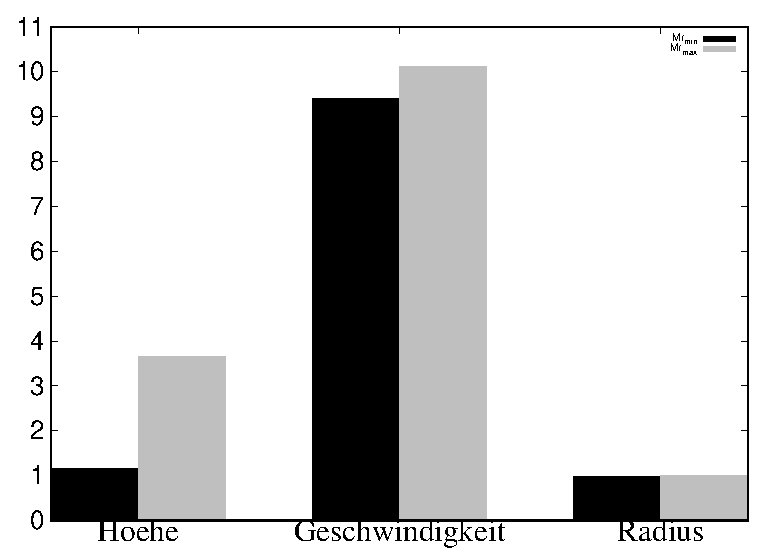
\includegraphics[width=0.4\linewidth]{pictures/gnuplot/3d/Hoehe/production/Auslenkungsfakt.eps} }}%
	\qquad
	\subfloat[Faktoren der Kraft]{{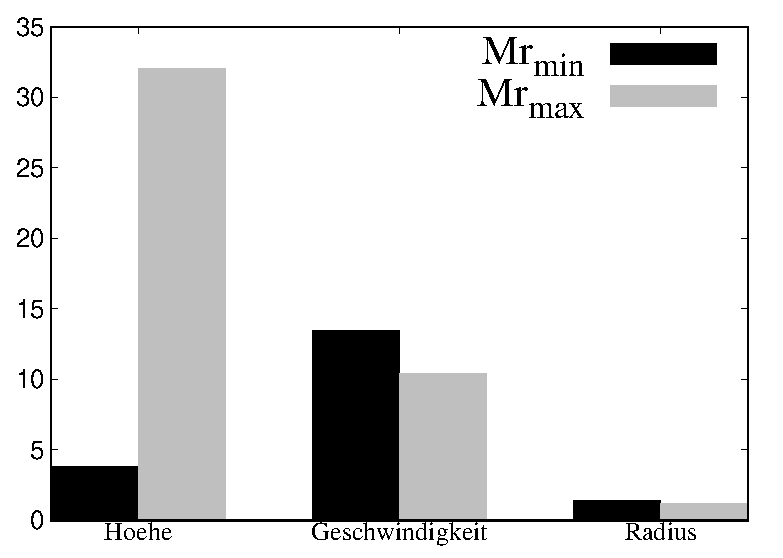
\includegraphics[width=0.4\linewidth]{pictures/gnuplot/3d/Hoehe/production/Kraftfakt.eps} }}%
	\caption{Faktoren: (v.L.n.R) Höhe, Geschwindigkeit und Radius}%
	\label{fig:Faktoren}%
\end{figure}

Wie in Abbildung~\ref{fig:Faktoren}(a) zu sehen ist, sind bei Höhe, Geschwindigkeit und Radius die Faktoren zwischen $Mr_{min}$ und $Mr_{max}$ ungefähr gleich. Zu erkennen ist jedoch, dass die Höhen- und die Geschwindigkeitsvariation verglichen mit dem Radius einen wesentlich größeren Einfluss aufweisen.
Die Auftreffstelle und das Seitenverhältnis wurden in Abbildung~\ref{fig:Faktoren} ausgelassen, da hier die Maxima der Kraft und Auslenkung nicht zwingend bei der unteren und oberen Schranke der Parameter auftritt. Ihre Signifikanz darf jedoch nicht außen vor gelassen werden.\\
Vor allem bei der Änderung der Auftreffstelle bilden sich interessante Trends aus. Die größte Auslenkung tritt bei ca. $\frac{\xi}{a} = \frac{\eta}{b} = 0.75$ auf. Da die Kraft auch an diesen Stellen am größten wird ist davon auszugehen, dass hier am wahrscheinlichsten Schäden nach einem Stoß entstehen. \\
Beim Seitenverhältnis biegt die Platte sich am meisten bei $1.6 \leq Sv \leq 3.5$ durch. Es scheint, dass Platten mit einem Seitenverhältnis von $Sv = 2.5$ am anfälligsten für Schäden durch Durchbiegung sind.

%ab hier finn

\section{Maximale Kraft}
\label{sec:Kraft}

Betrachtet man die maximal auftretende Kraft, sieht man, dass hier die Höhe und die Geschwindigkeit den größten Einfluss haben. Aus Abbildung~\ref{fig:Faktoren}(b) kann man ablesen, dass die Faktoren des Radius, analog zur Auslenkung, zwischen der minimalen und maximalen Kraft bei $Mr_{min}$ und $Mr_{max}$ verglichen mit den Faktoren der Höhe und der Geschwindigkeit gering sind. \\
Am signifikantesten verändert sich die Kraft bei der Variation der Plattenhöhe $h$. Hier liegt ein Kraftunterschied von $P(Mr_{max}) \; \approx \; 8 \cdot P(Mr_{min})$ vor. Dies ist auf die Potenz der Höhe in $\overline{a}$ in Kapitel~\ref{chap:Principles} zurückzuführen. \\
Auch die Auftreffgeschwindigkeit hat einen großen Einfluss auf die auftretende Kraft. Da das Modell ohne Dissipation rechnet, entsteht dieser Einfluss direkt aus der Energiegleichung, in die $v_{0}$ quadratisch eingeht. \\
Bei der Variation des Auftreffortes und des Seitenverhältnisses die größten Kräfte an den selben Stellen wie bei der Auslenkung auf.\\
Da die auftretenden Kräfte bis in den Mega-Newton Bereich gehen, müssen diese bei der Schadensbeurteilung dringend berücksichtigt werden.

\section{Ausblick}
\label{sec:Ausblick}

Wie in dieser Arbeit beschrieben, haben vor allem die Plattenhöhe, die Auftreffgeschwindigkeit und die Auftreffstelle einen großen Einfluss auf das beschriebene Problem. Bei der Schadensbeurteilung sollten diese drei Faktoren berücksichtigt werden. Auch das Seitenverhältnis $Sv$ hat einen signifikanten Einfluss, jedoch sind die Ergebnisse durch die auftretenden numerischen Instabilitäten nur bedingt verlässlich. In diesem Bereich kann in zukünftigen Arbeiten weitere Recherche betrieben werden. \\
Ein weiteres Forschungsthema liegt in dem Bereich der dünnen Platten mit $h \leq 0.5 [cm]$. In diesem Bereich ist das Skript mathematisch nicht mehr stabil und kann numerisch nicht mehr gelöst werden. Da oftmals dünne Platten aus Gewichtsgründen verbaut werden, sind hier weitere Überlegungen gefragt. \\


